\section{Selection Efficiencies}
\label{sec:selection}

As a summary of the previous sections, the cut flow of the analysis is as follows:
\begin{itemize}
\item At least two photons and two jets in the event
\item At least two photons pass the trigger based pre-selection (see sec. \ref{sec:trigger});
\item At least two photons pass the kinematic and identification requirements (see sec. \ref{sec:photons}) $\to$ select two highest $E_{T}$ photons as diphoton candidate;
\item At least two jets pass the kinematic selection (see sec. \ref{sec:jets}) $\to$ select two jets with highest b-tagging score as dijet candidate;
\item Event can be classified in either High Purity Category or Medium Purity Category;
\end{itemize}

The efficiency after each step above and taking into account the acceptance is estimated and shown for each of the signal samples considered in our analysis. Figure~\ref{fig:cutflow-signal-Graviton} shows the cut flow efficiency$\times$acceptance  for the graviton signal samples ranging from mass hypothesis of 250 up to 900 GeV on the top left. It shows the one with the bjet regression applied, on the top right and the ratio of the efficiencies of the two on the bottom.
figure~\ref{fig:cutflow-signal-Radion} shows the analog cut flow efficiency$\times$acceptance of the Radion samples (with mass range of 250 to 900 GeV) on the top left. It shows the same cutflow with the bjet regression applied, on the top right and the ratio of the efficiencies of the two on the the bottom.
Figure~\ref{fig:cutflow-signal-NR-mva} and figure~\ref{fig:cutflow-signal-NR-wRegression}  show the analog cutflow$\times$acceptance of the 14 nodes of  nonresonant signal  benchmarks corresponding to  12 anomalous couplings  combinations, in addition to the box diagram(node=0) and the SM couplings (node=1) as defined in  subsection~\ref{sec:nonresMC} and in table~\ref{tab:bench}. Figure~\ref{fig:cutflow-signal-NR-mva} displays the values for the cut based categorization on the top left, the ones with the MVA based categorization on the top right and the ratios of the two on the bottom. Figure~\ref{fig:cutflow-signal-NR-wRegression} shows the values when the b-jet regression is applied in addition the MVA based categorization in the left, and the ratio of the two.


These figures report results using for the above described selections where the  photon identification is the $\Hgg$ MVA procedure.

%We also performed the selection using the cut based photon identification. The ratio of the efficiencies is performed to assess the performance difference between the different photon Id. The result of the comparison is shown in top figure~\ref{fig:cutflow-signal-diff-CutB} and bottom figure~\ref{fig:cutflow-signal-diff-CutB} for Graviton and Radion samples, respectively. The performance of the EGamma MVA photon identification outrates the one of the cut based photon Id., by 10. to 15. \% at low resonance masses, and is around 8-10\% for high resonance masses. \\
%Although we performed a detail study of the MVA photon id. and shown that we could choose a different WP from EGamma MVA(see table~\ref{tab:MVA-WP}), the efficiency for the latter is expectedly  better as shown in figure~\ref{fig:cutflow-signal-diff-MVAEG}.\\
%A comparison of the Graviton and Radion signal efficiencies is also performed in figure~\ref{fig:cutflow-signal-diff-RG}. It is shown that Graviton samples show a better efficiency, more than 10\% higher for high masses.

\begin{figure*}[thb]
  \centering
  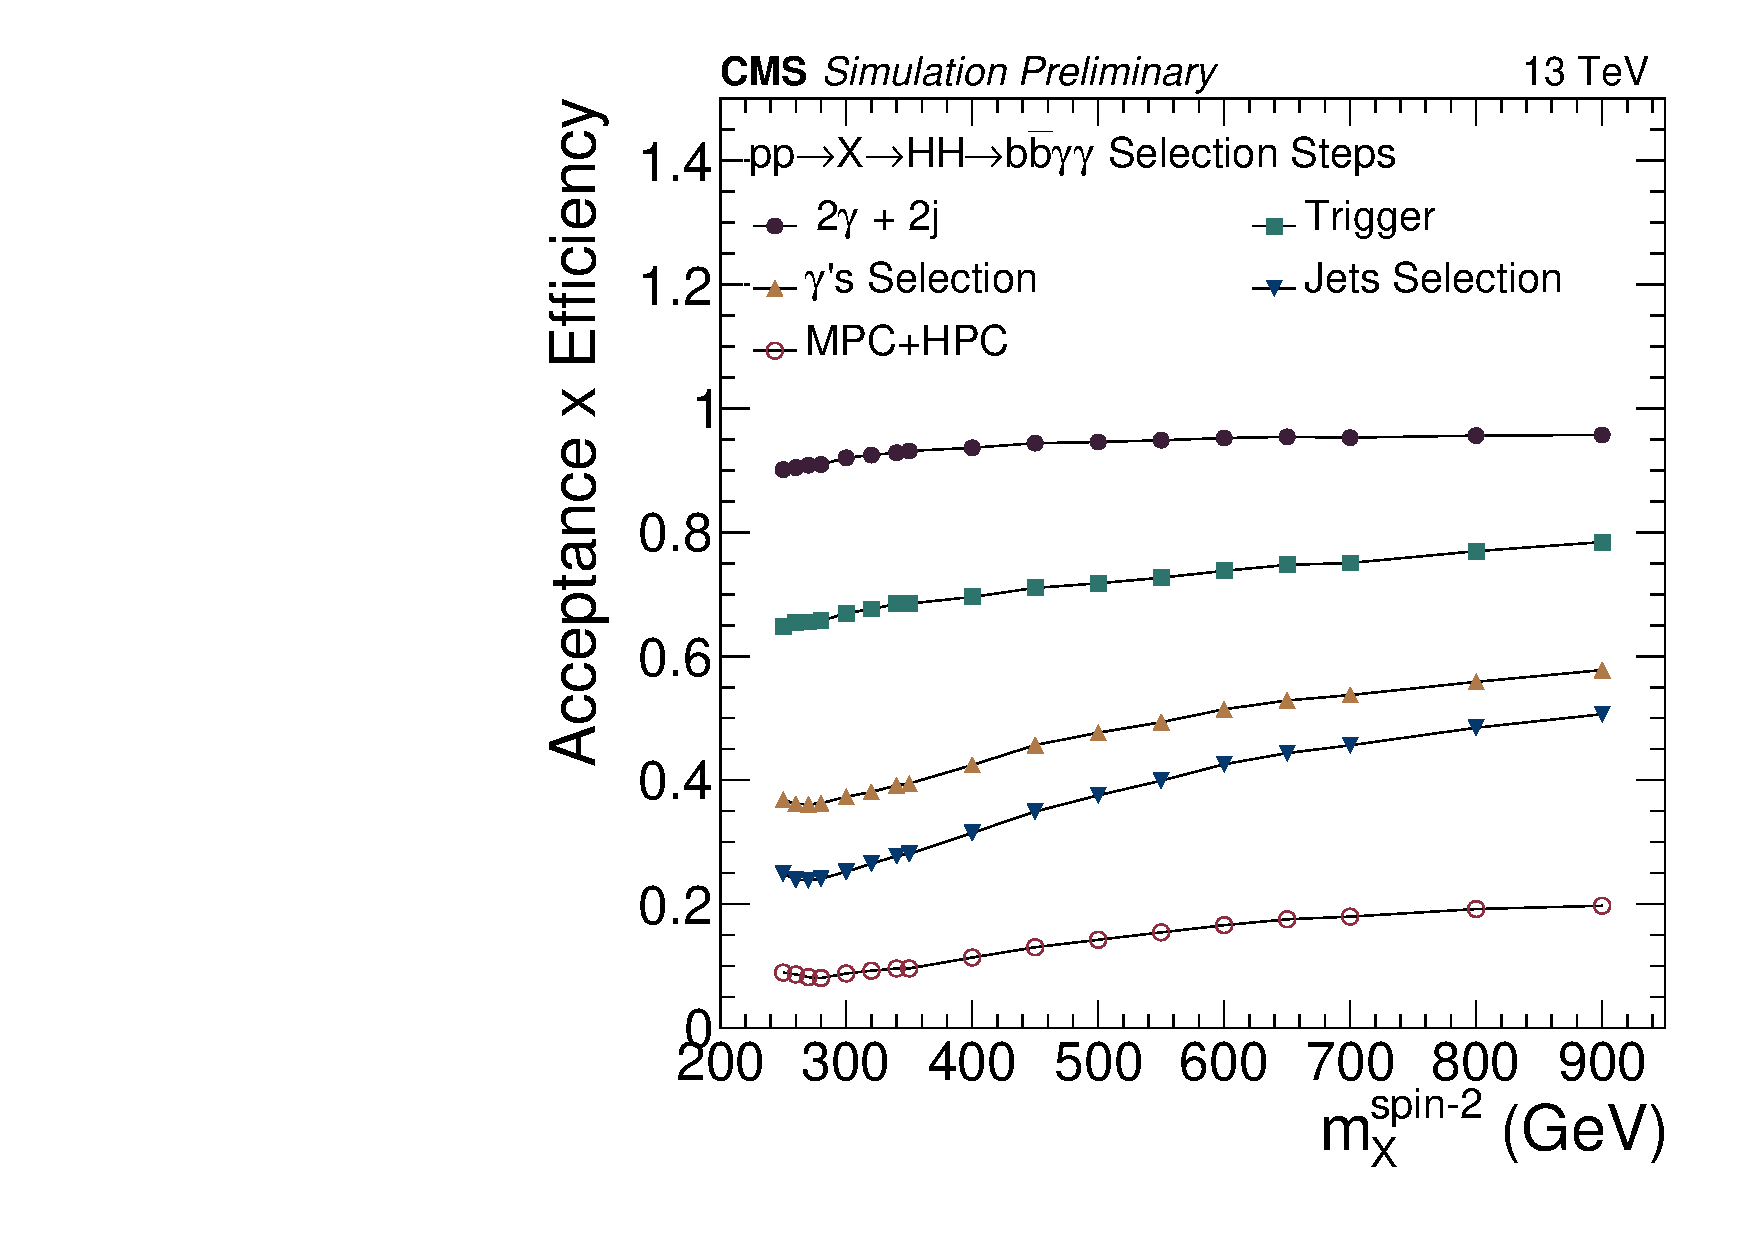
\includegraphics[width=0.45\textwidth]{figures/sec-efficiency_plots/res_effs_Graviton.pdf}\hfil
  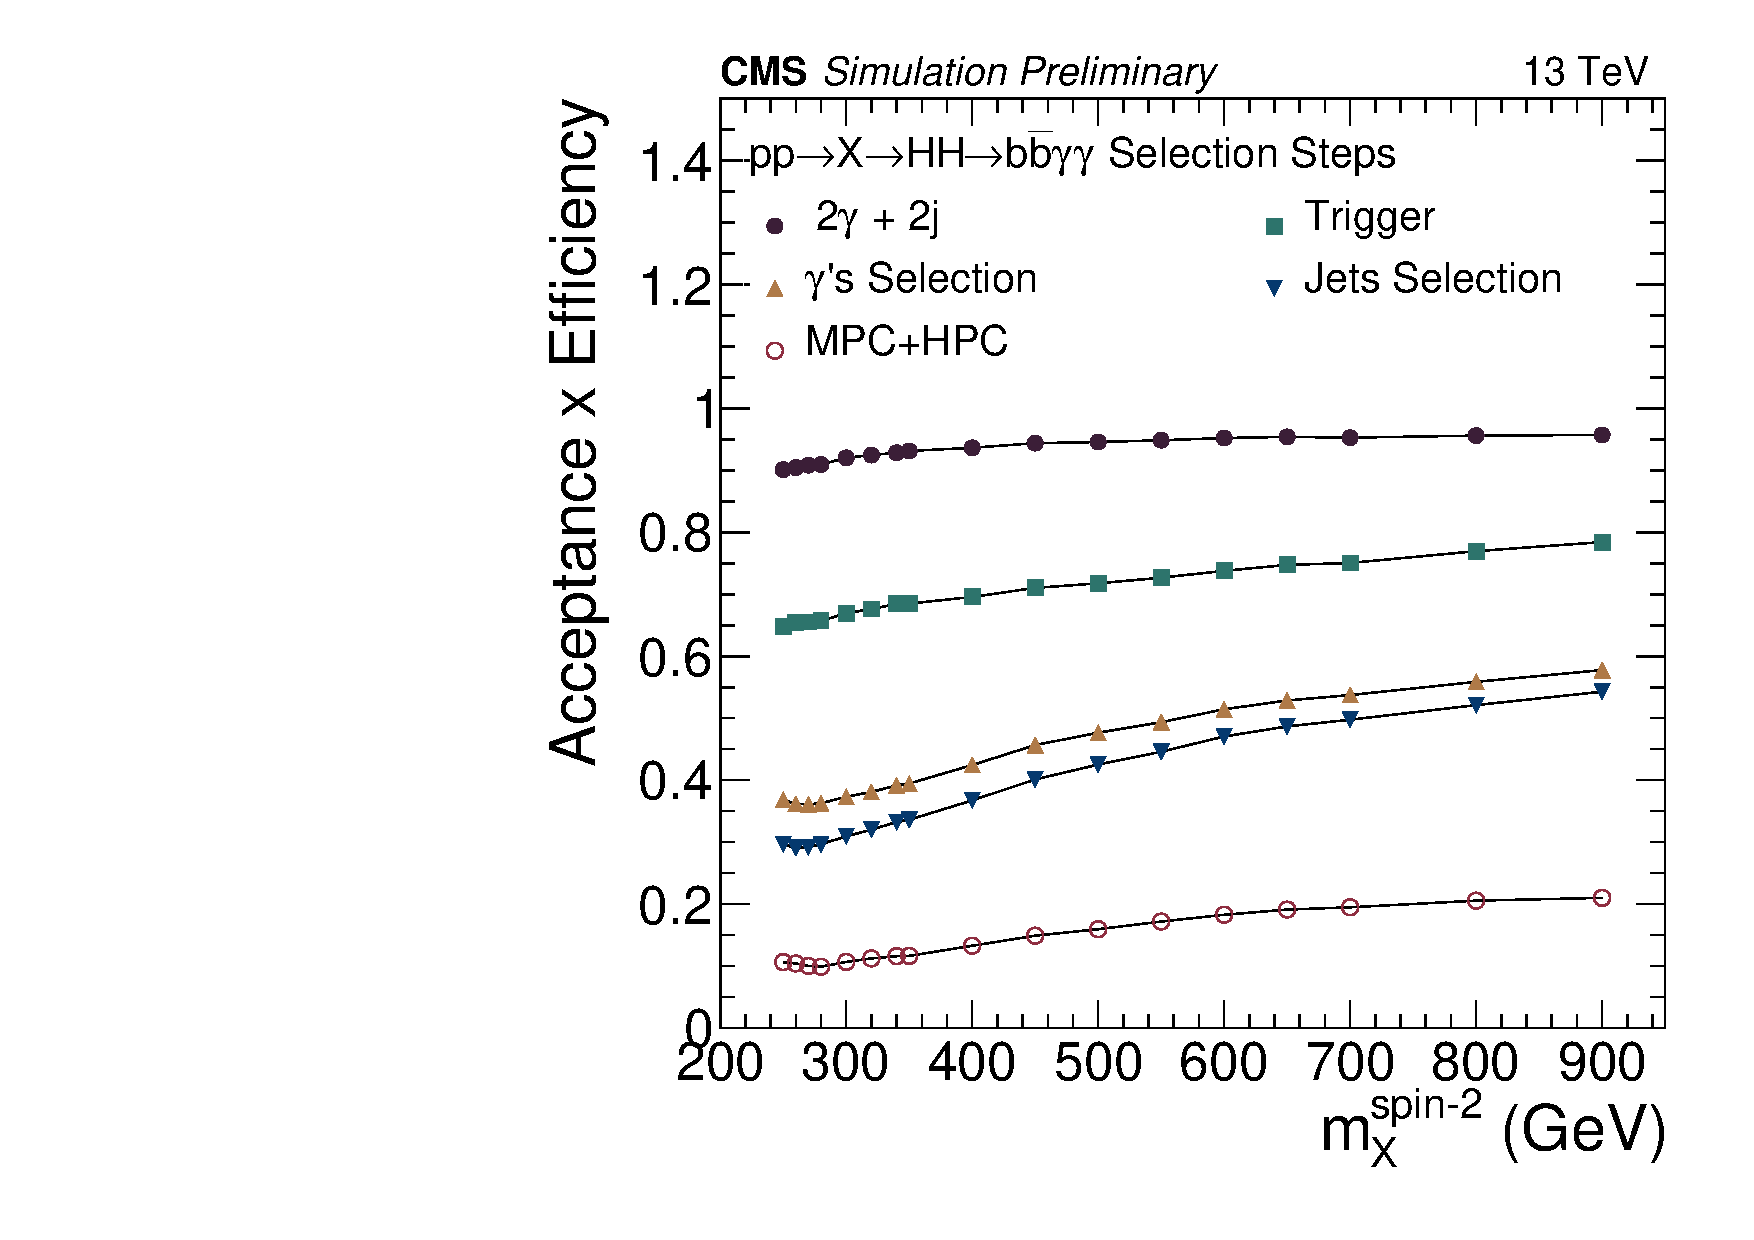
\includegraphics[width=0.45\textwidth]{figures/sec-efficiency_plots/wRegression/res_effs_Graviton_reg.pdf}\hfil
  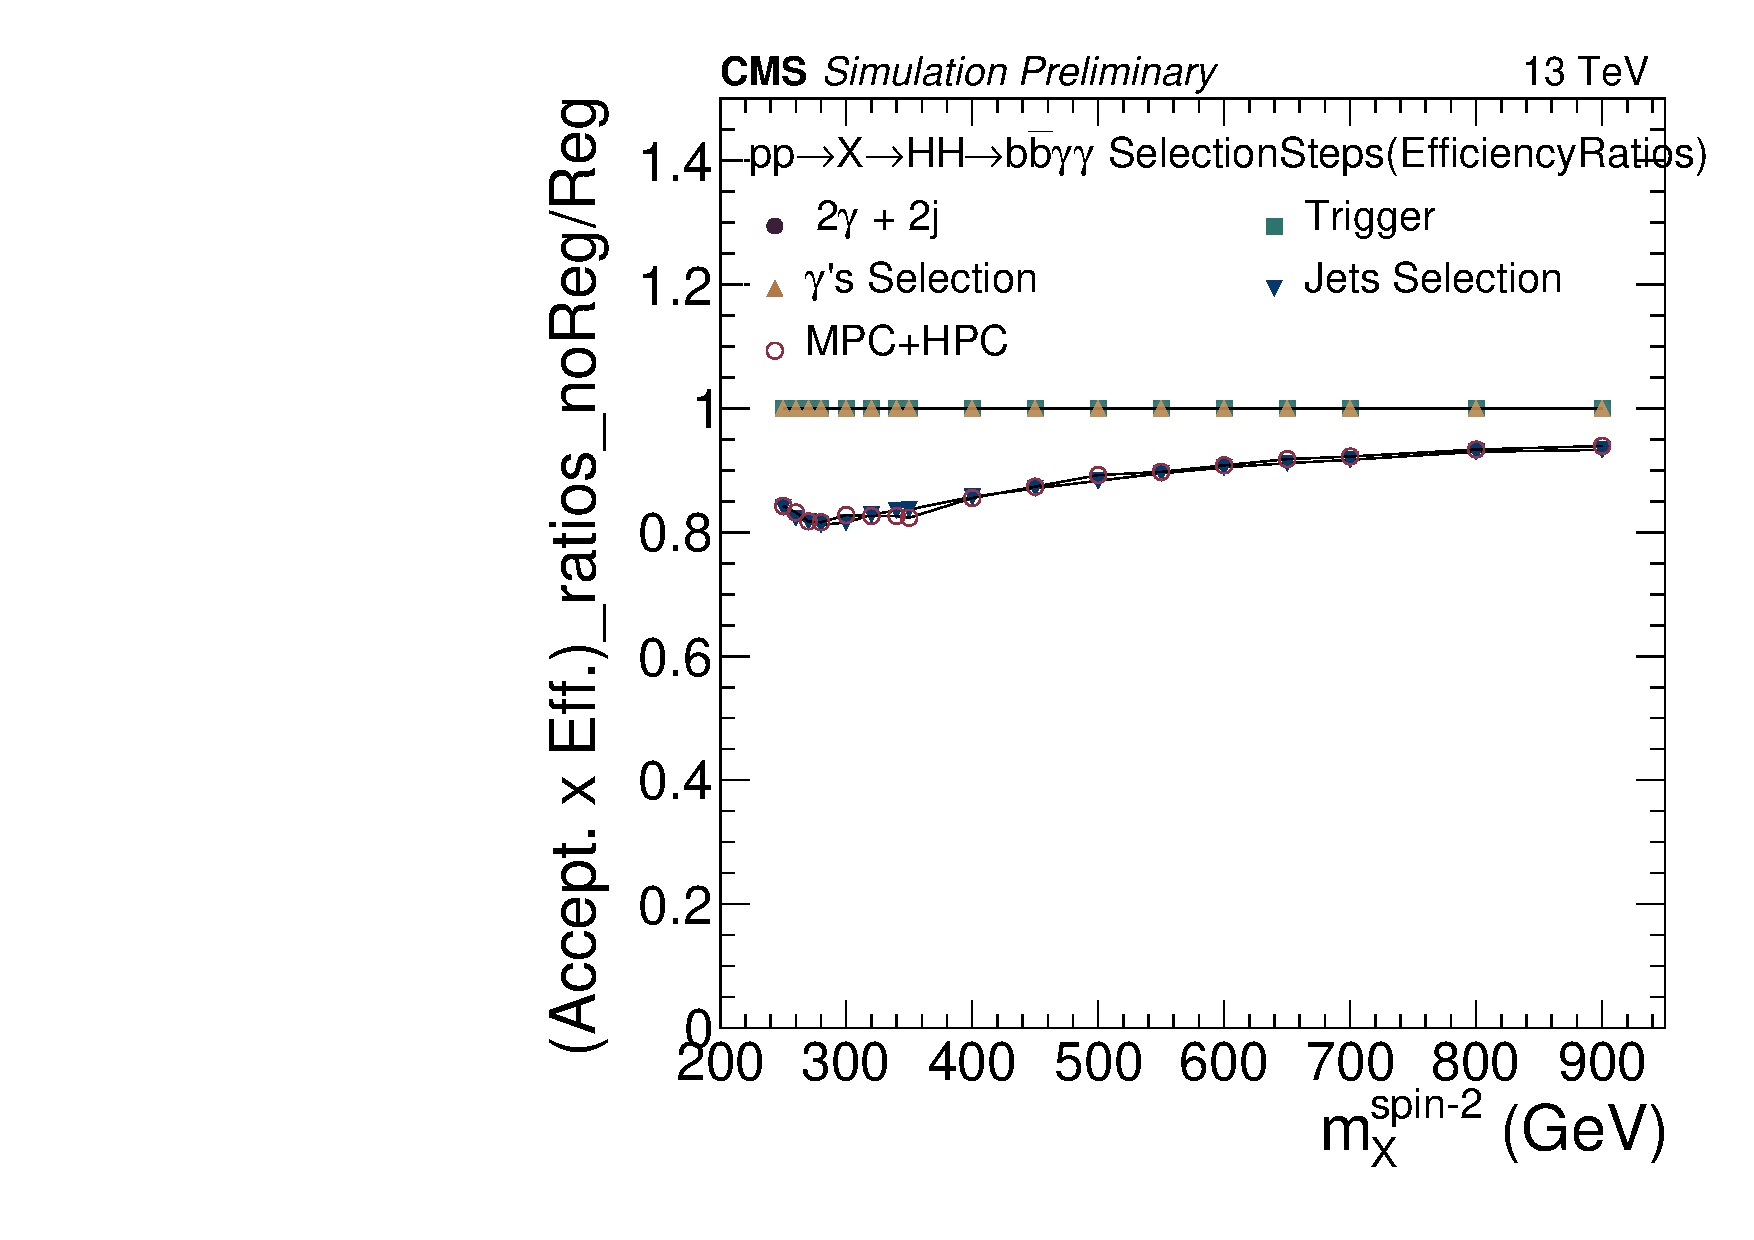
\includegraphics[width=0.45\textwidth]{figures/sec-efficiency_plots/wRegression/res_effs_Graviton_regRatio.pdf}\hfil
  \caption{Graviton signal acceptance$\times$efficiency for each cut (described in text) on the top left plot, the bjet regression is applied on the top right  and the ratio of the cutflows on  the bottom.}
  \label{fig:cutflow-signal-Graviton}
\end{figure*}


\begin{figure*}[thb]
  \centering
  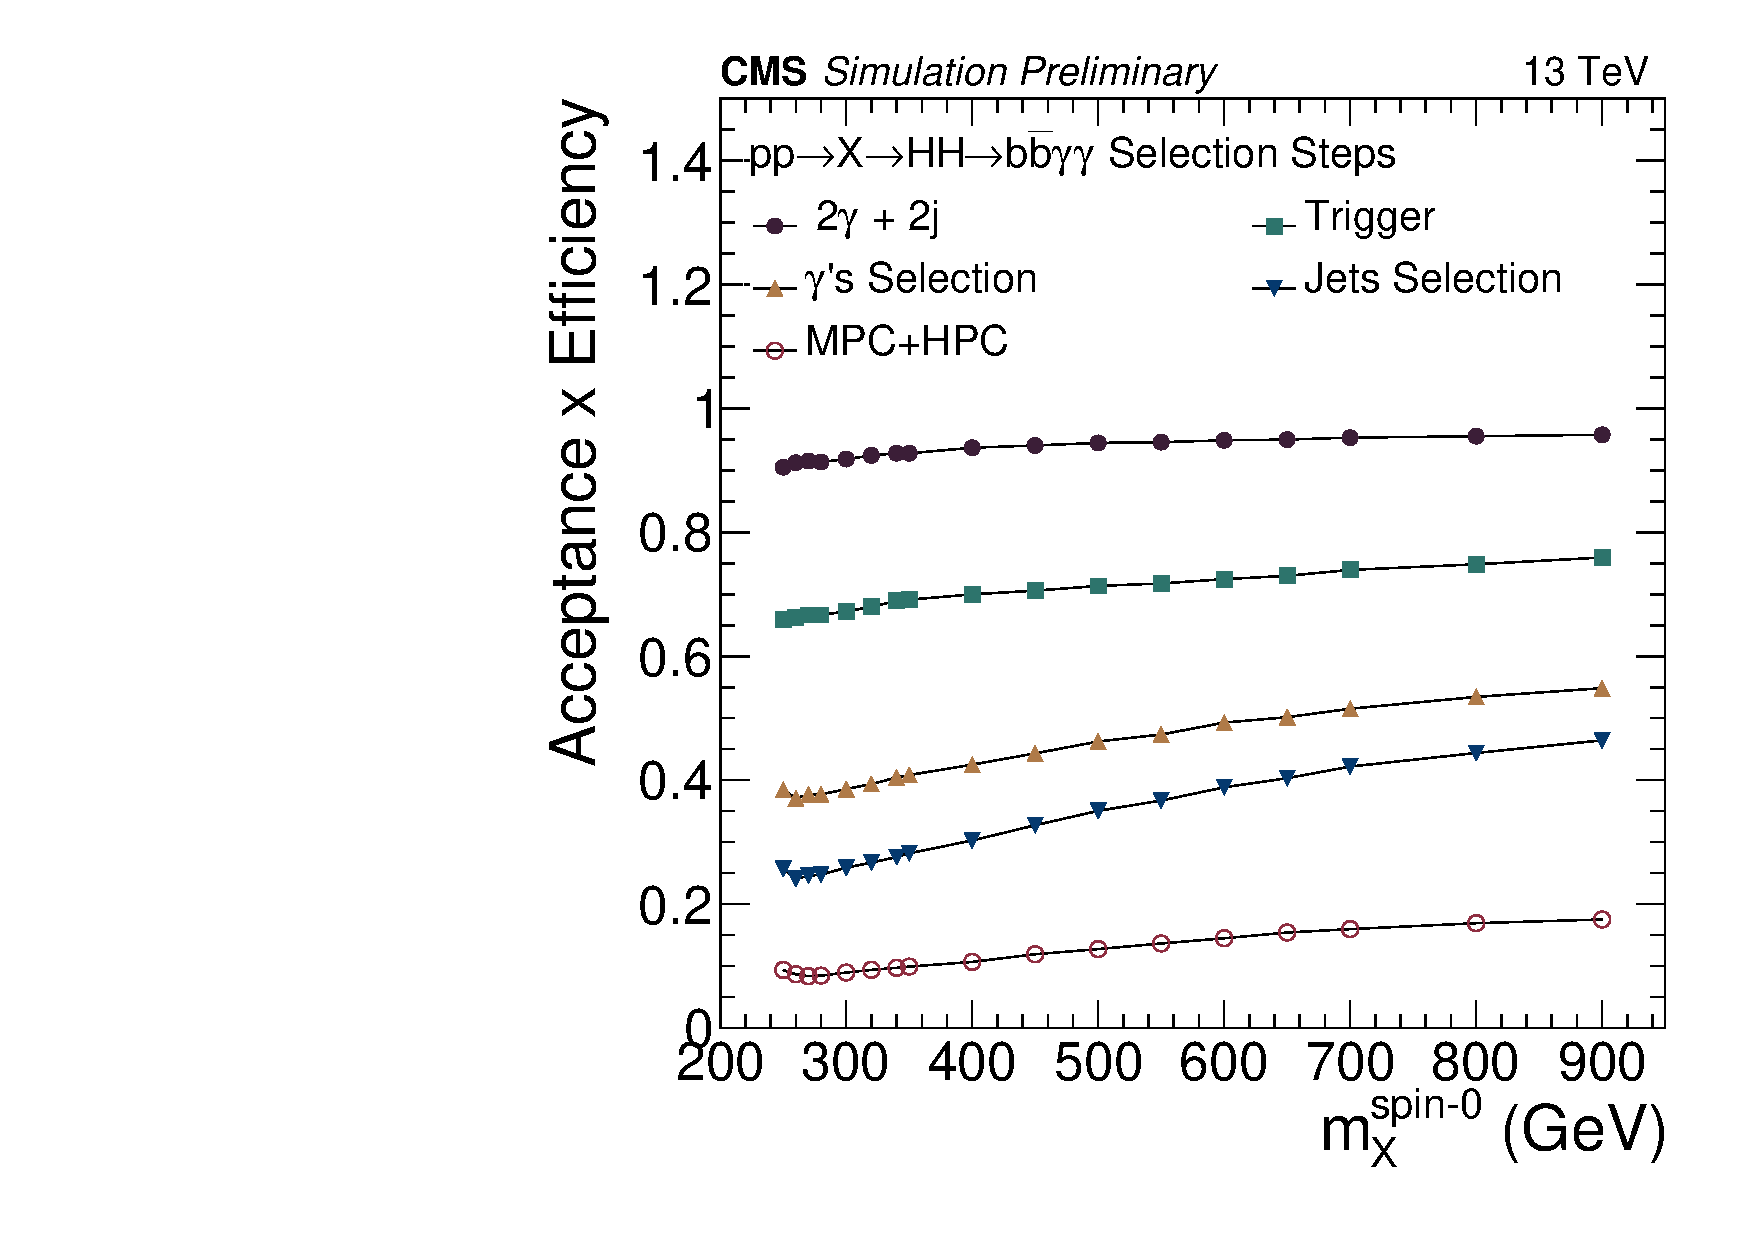
\includegraphics[width=0.45\textwidth]{figures/sec-efficiency_plots/res_effs_Radion.pdf}\hfil
  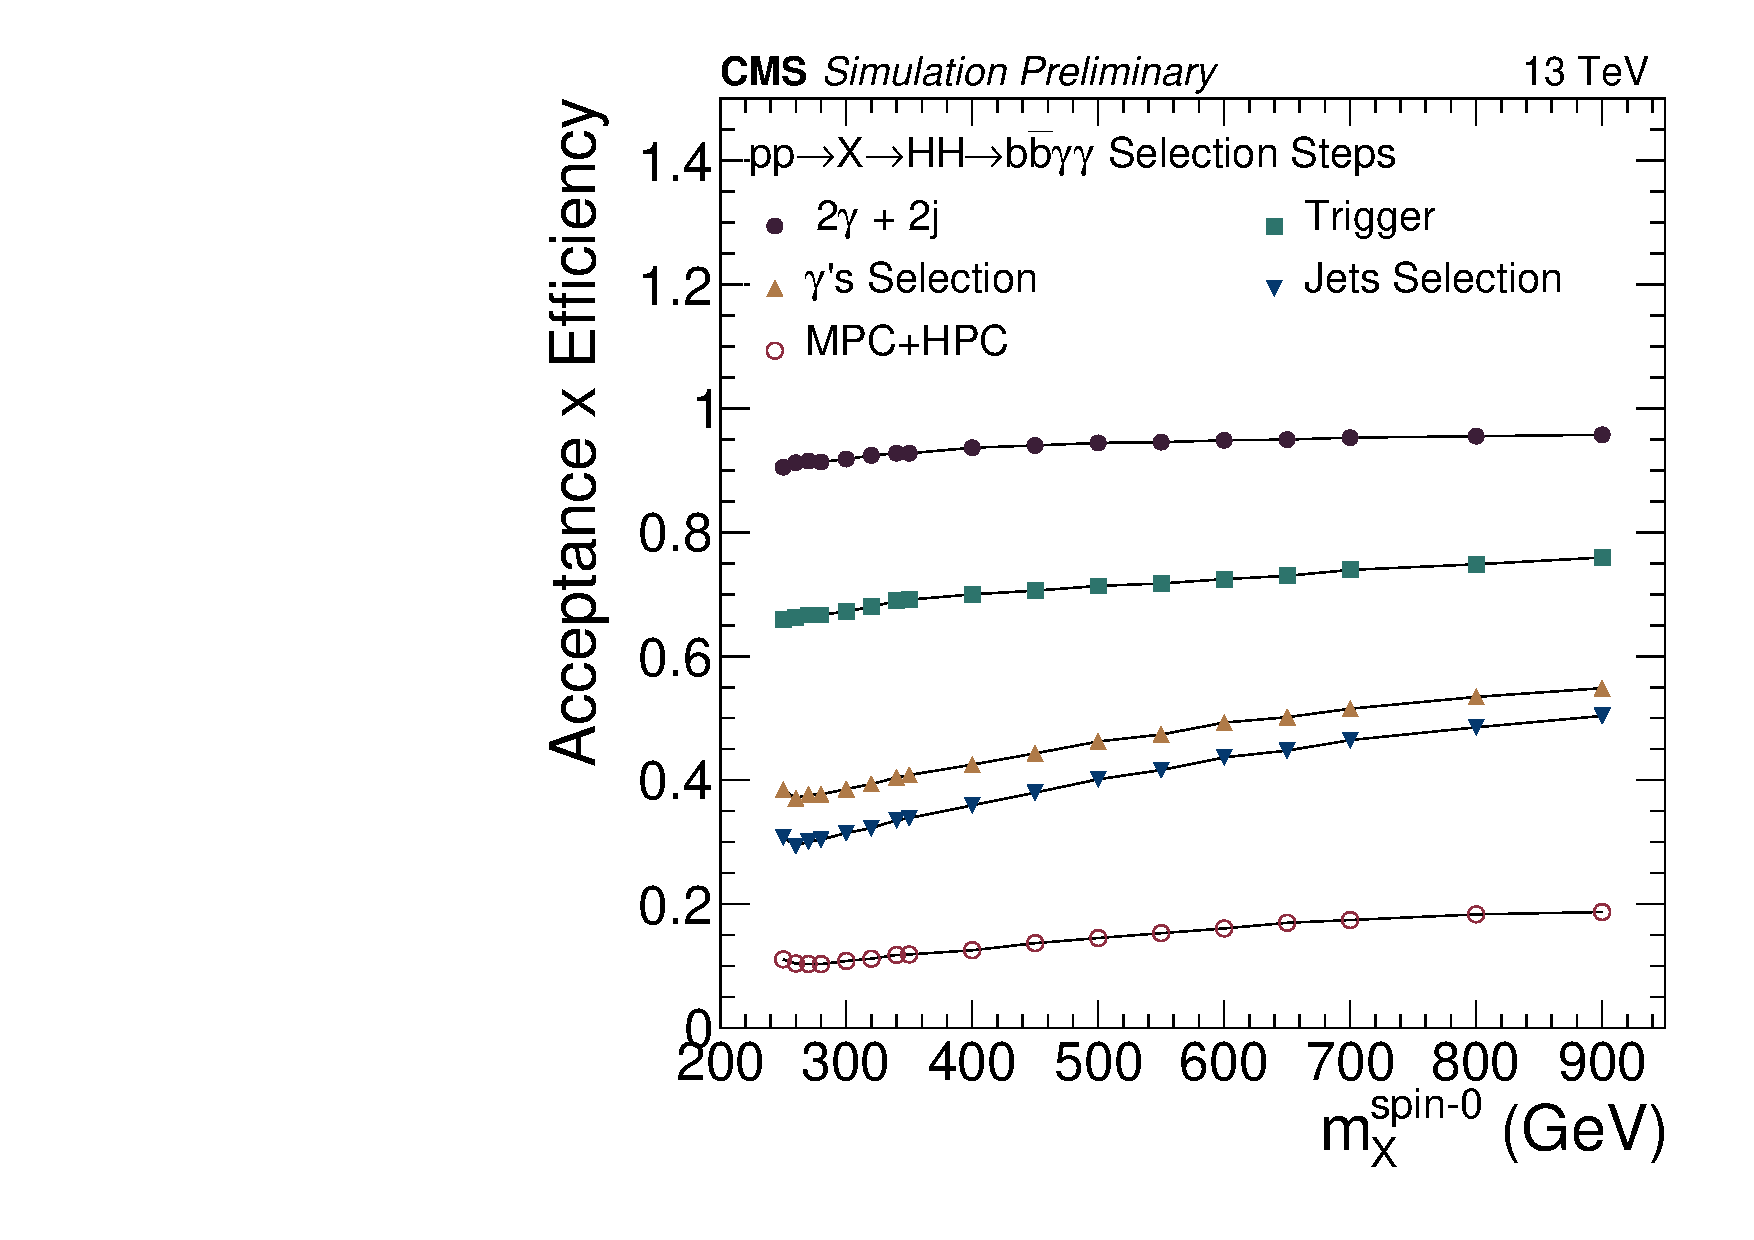
\includegraphics[width=0.45\textwidth]{figures/sec-efficiency_plots/wRegression/res_effs_Radion_reg.pdf}\hfil
  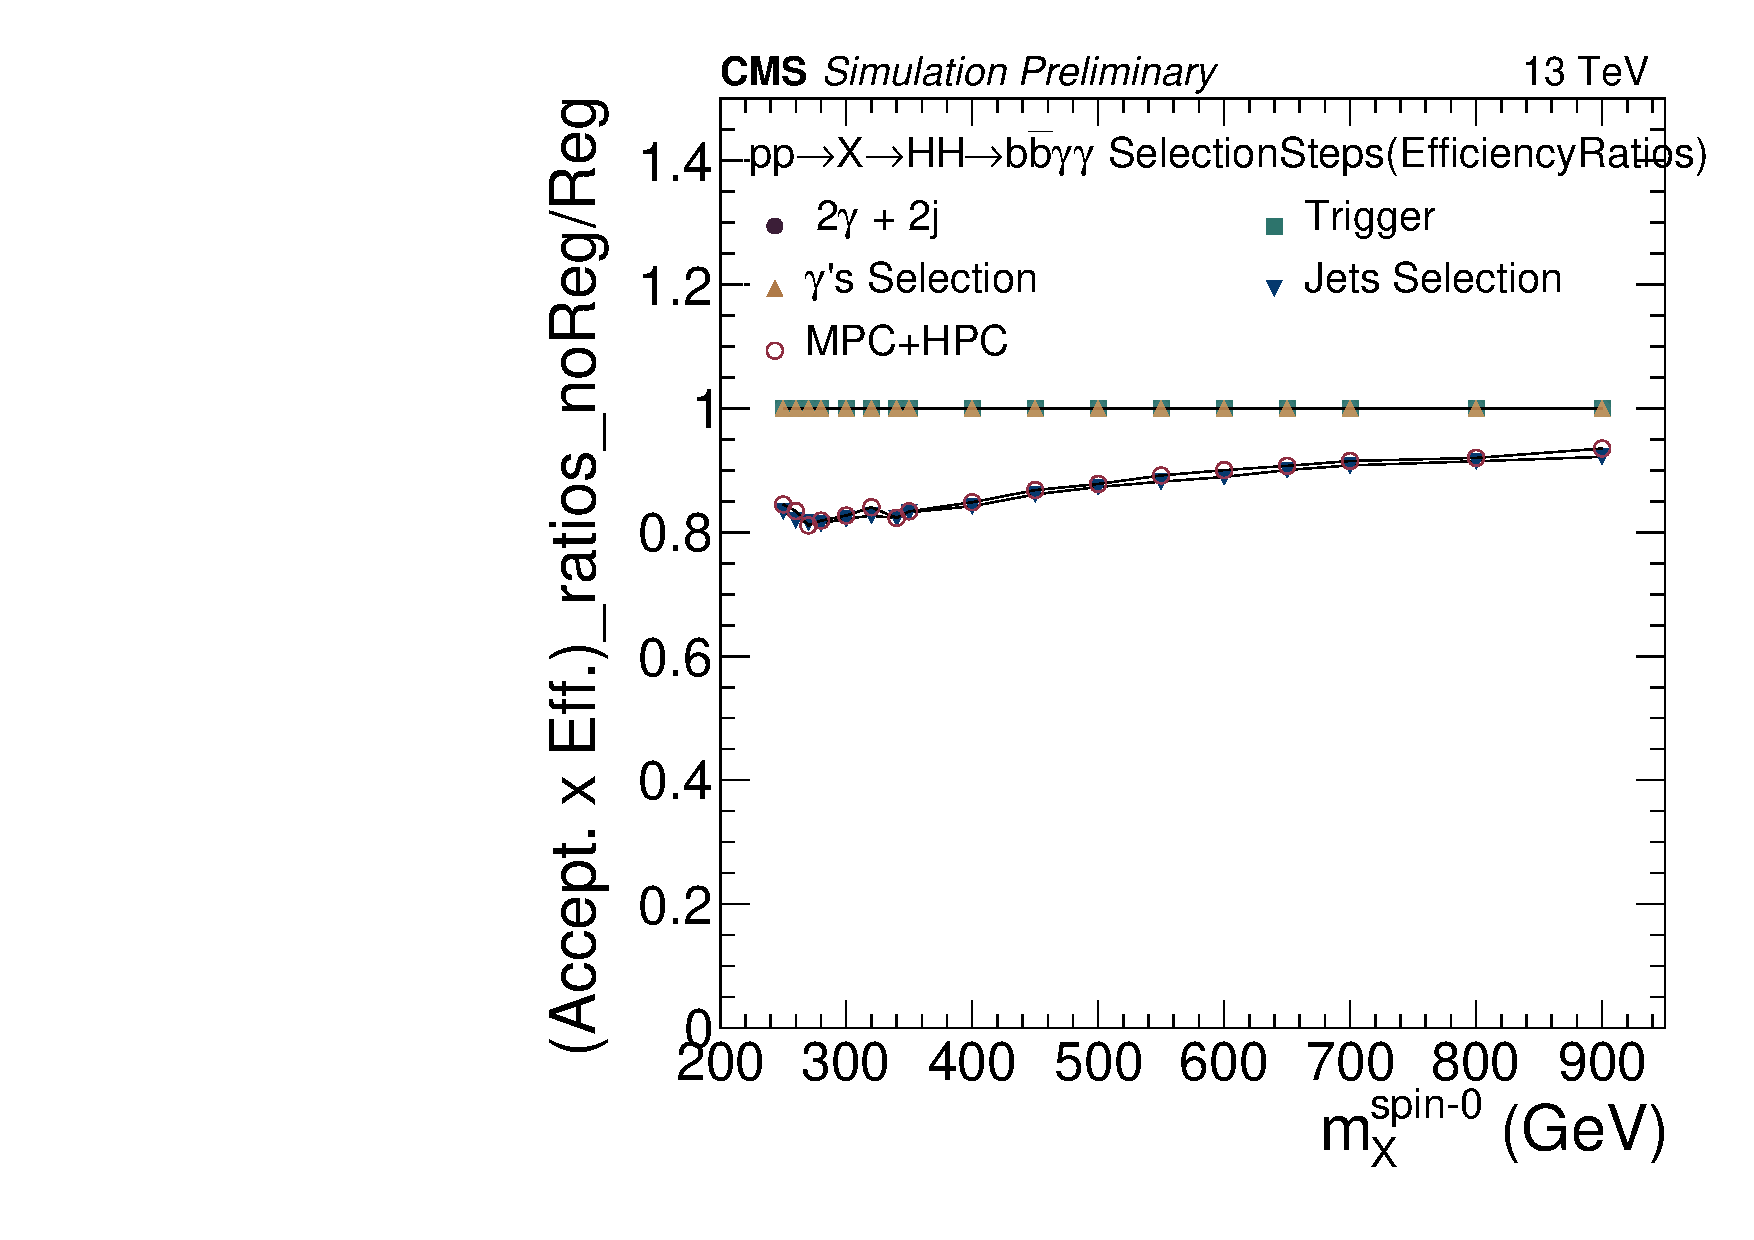
\includegraphics[width=0.45\textwidth]{figures/sec-efficiency_plots/wRegression/res_effs_Radion_regRatio.pdf}\hfil
  \caption{Radion signal acceptance$\times$efficiency for each cut (described in text) on the top left plot, the bjet regression is applied on the top right and the ratio of the cutflows on the bottom.}
  \label{fig:cutflow-signal-Radion}
\end{figure*}

\begin{figure*}[thb]
  \centering
  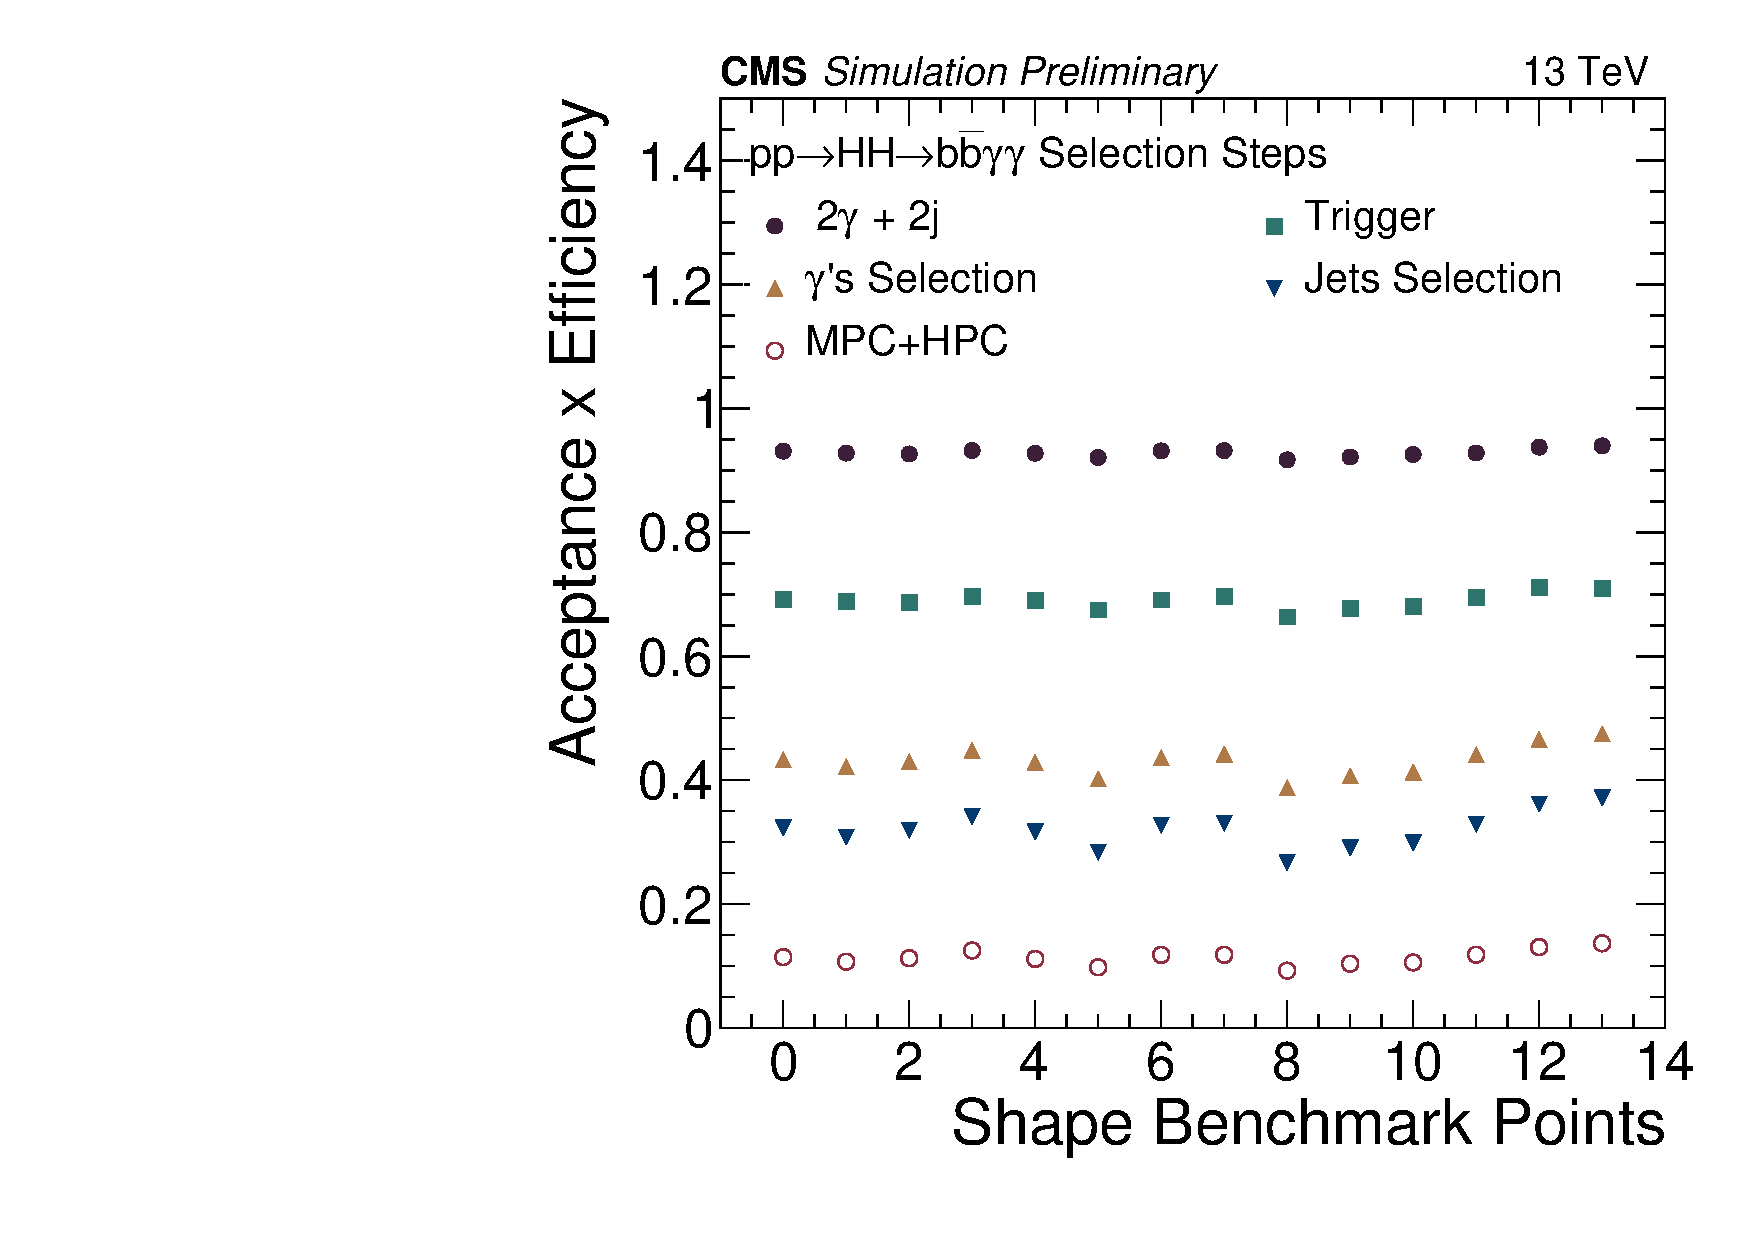
\includegraphics[width=0.45\textwidth]{figures/sec-efficiency_plots/nonres_effs.pdf}\hfil
  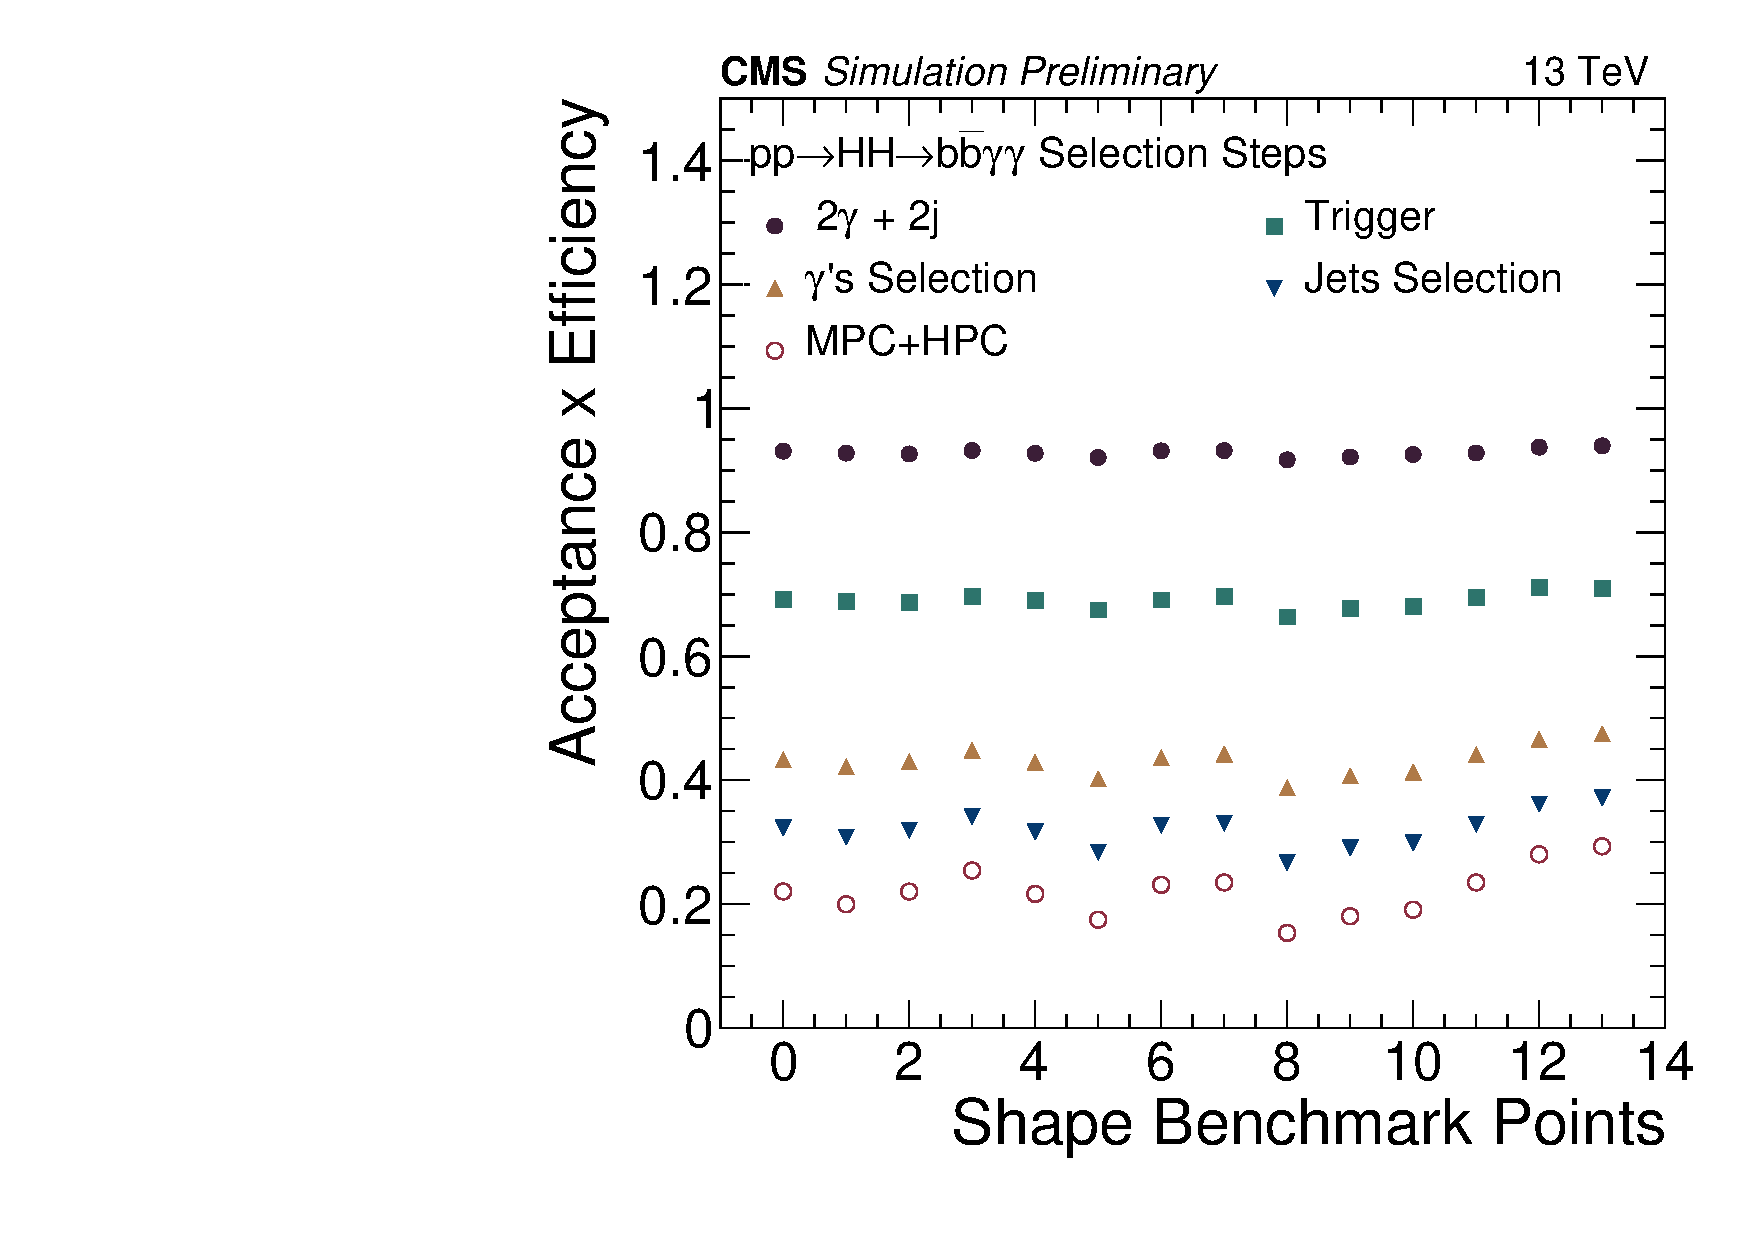
\includegraphics[width=0.45\textwidth]{figures/sec-efficiency_plots/nonres_effs_HHtagger.pdf}\hfil
  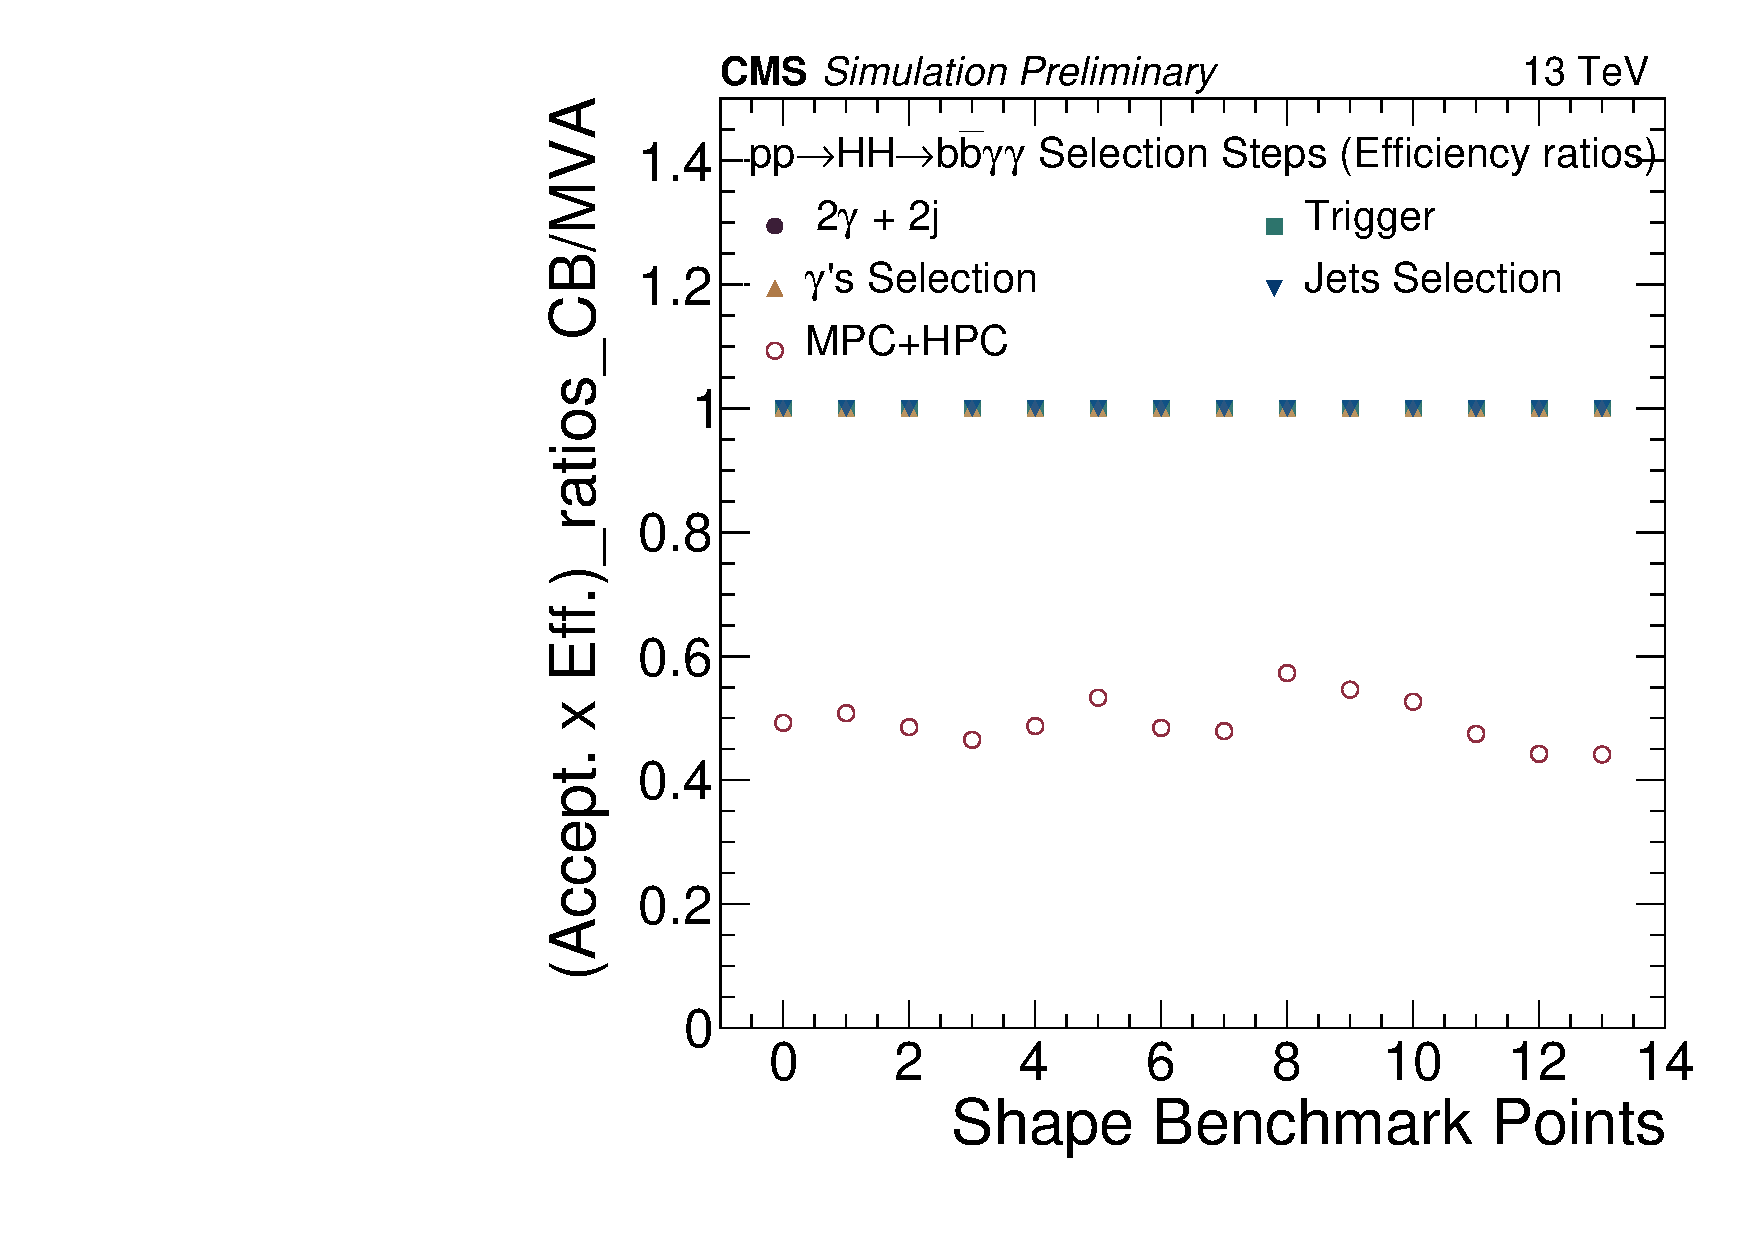
\includegraphics[width=0.45\textwidth]{figures/sec-efficiency_plots/nonres_effs_Ratio_CutBased_MVAHHTagger.pdf}\hfil
  \caption{Non-resonant acceptance x efficiency. Cut based categorization on the top left, MVA based categorization on the top right (analysis version) and the ratio of the two on the bottom.}
  \label{fig:cutflow-signal-NR-mva}
\end{figure*}

\begin{figure*}[thb]
  \centering
  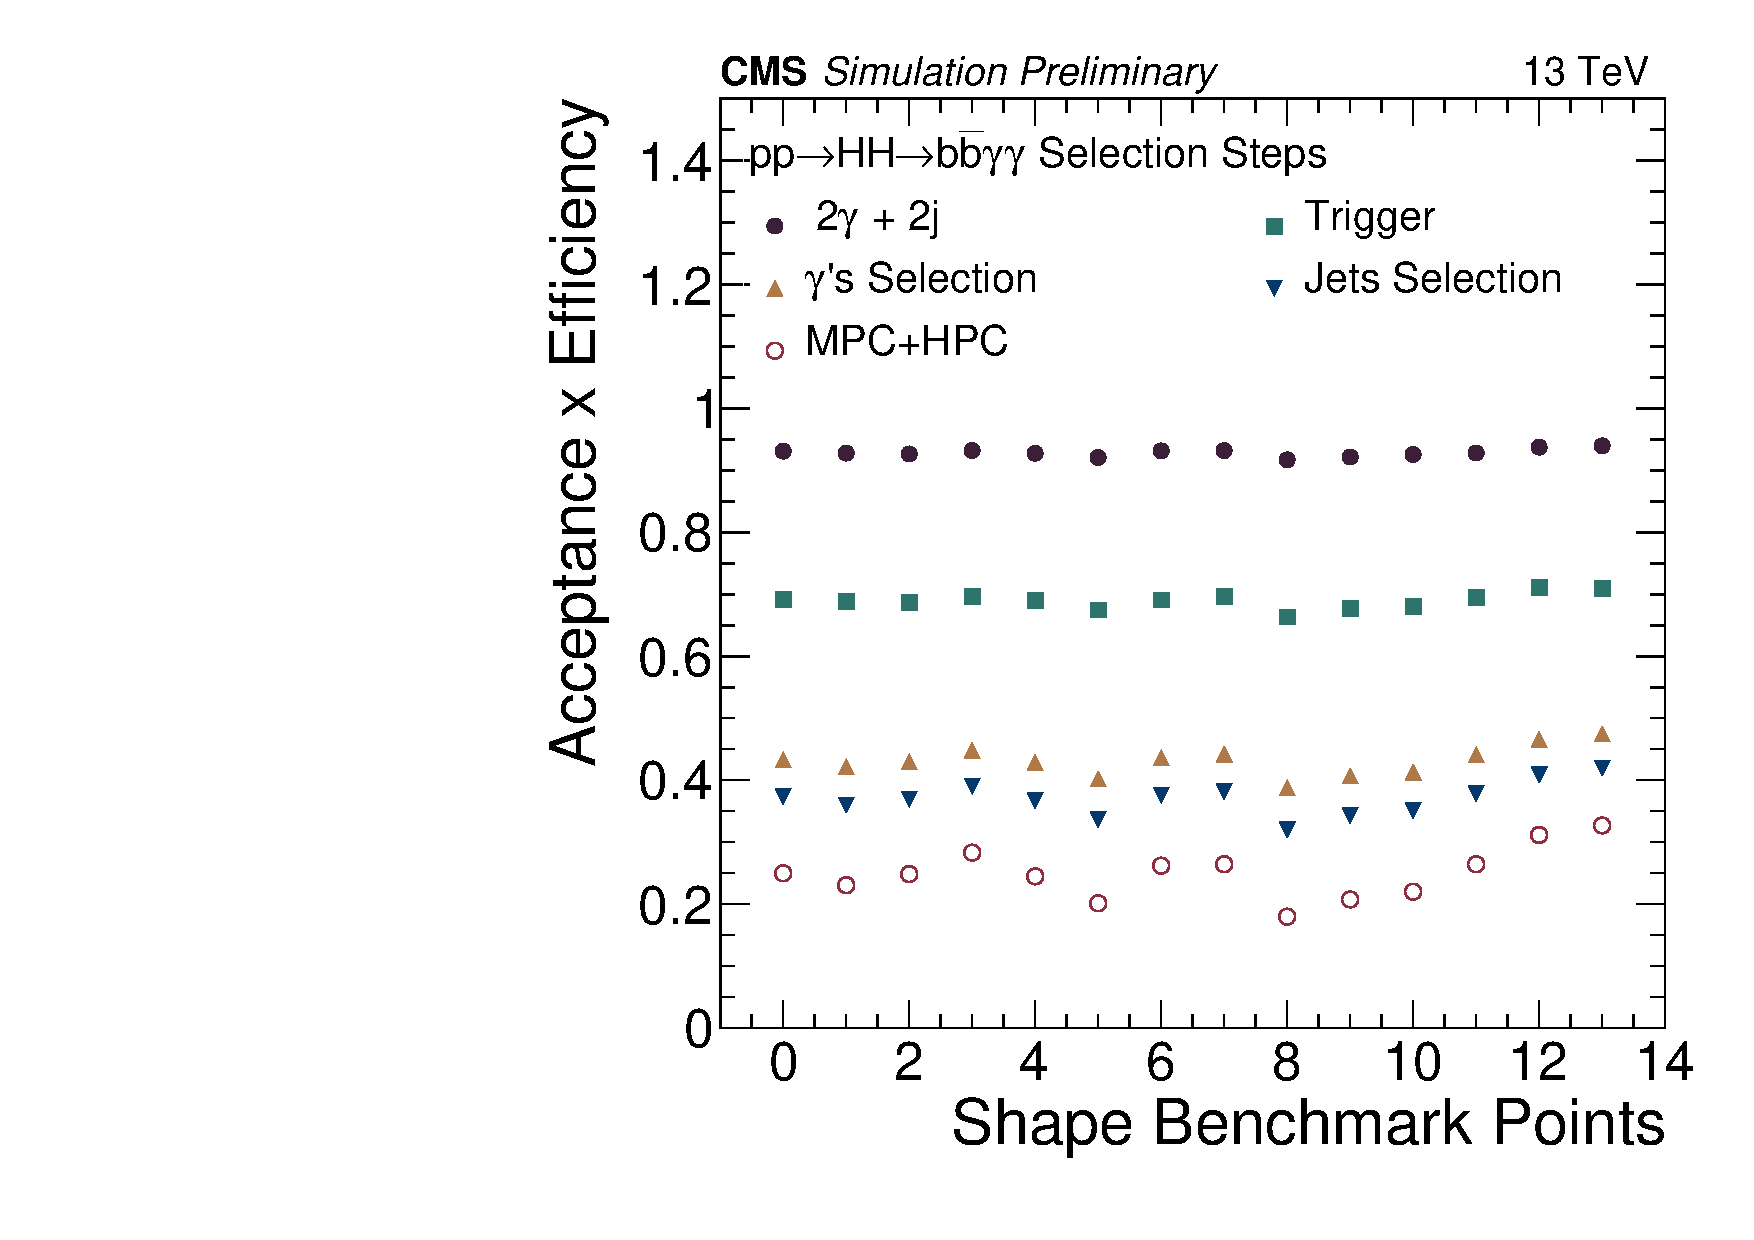
\includegraphics[width=0.45\textwidth]{figures/sec-efficiency_plots/wRegression/nonres_effs_reg.pdf}\hfil
  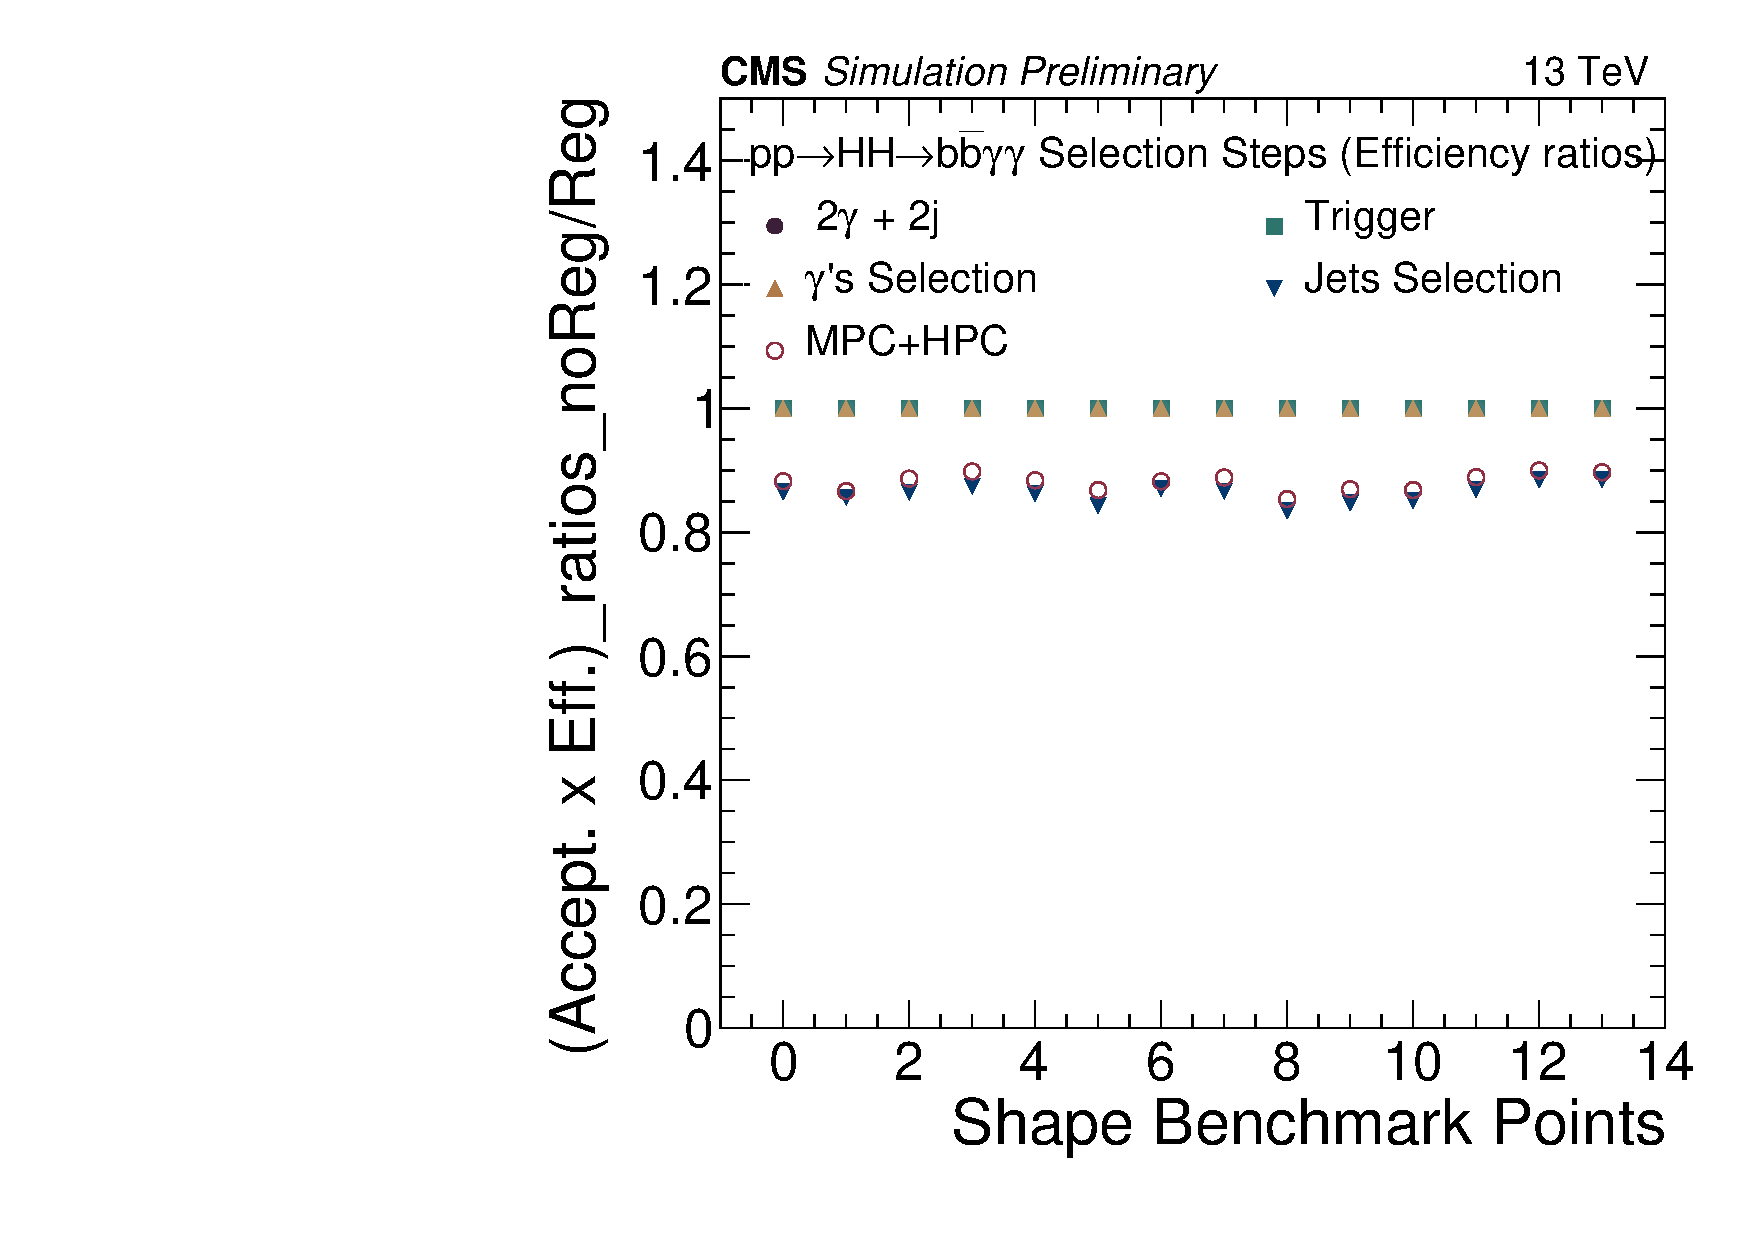
\includegraphics[width=0.45\textwidth]{figures/sec-efficiency_plots/wRegression/nonres_effs_reg_Ratio_MVAHHTagger_reg.pdf}\hfil
  \caption{Non-resonant acceptance x efficiency. Jet energy regression applied in addition to MVA based categorization on the left, ratio (bjetReg.+MVA)/MVA on the right (analysis version).}
  \label{fig:cutflow-signal-NR-wRegression}
\end{figure*}


